% Chapter 2

\chapter{PESTE} % Chapter title

\label{ch:examples} % For referencing the chapter elsewhere, use \autoref{ch:examples} 

%----------------------------------------------------------------------------------------


\section{Political environment}
\subsection{Educational policy} \graffito{opportunity}

\noindent Education is considered very important in Switzerland.\footnote{test} Therefore everything that is considered valuable in this area is usually supported (if not financially then at least morally). A commonly envisioned goal of the Swiss education system is to form «active» citizens who develop their skills in media and multilingualism. This coincides nicely with what the project offers.\autocite{zukunft-bildung},\autocite{oecd-pisa2009}

\subsection{Interest Groups inside of the School opportunity} \graffito{menace}
\noindent
The multiple actors and interest groups inside of the school may see the project favorably or not. Depending on the general opinion, the project may be hampered or receive tailwind. \autocite{cormen:2001}
\paragraph{}
\emph{Language Teachers} might view the project as a competitor and therefore oppose or at least ignore it.
\paragraph{}
Other groups like \emph{BALEINEV}, \emph{AGE} and the \emph{sports group} seem to look at it more favorably. They consider it a platform to promote their own interests.\footnote{This information was directly obtained from the respective groups, which expressed their interest.}


\section{SWOT-Analysis}
\subsection{SWOT-Matrix}

\begin{tabu}{|l|X[1]|X[1]|}

\hline
 			& Positive & Negative \\ \hline
 Internal	&
 			\textsc{Strengths}
Very low running costs. Allow offering the podcast for free and minimizing the risk for the listener.
Knowledge transfer. Great pool of competencies and an environment which supports sharing ones knowledge.
			&
			Weaknesses
Ideas as primary matter. Makes it difficult to assure quality and procurement.
Dependency on external platforms to provide the content. Without
any warranties, a big part of the distribution is at the mercy of these providers. \\
\hline

External 	&
			Opportunity
Doers attitude of the students.
Provides a source of potential participants.
Low prices for equipment. Provides the participants with high quality hard- and software and helps to create the best possible product.
			&
			Threat \citeauthor{bentley:1999}
Lack of a participatory culture. Would dry up the flow of new participants and therefore the most important resource and customer.
Opposition by other groups within the school. Could slow down everything and finally make the project untenable. \\
\hline

\end{tabu}



\lipsum[1]

%----------------------------------------------------------------------------------------

\section{A New Section}

\lipsum[2]

Examples: \textit{Italics}, \spacedallcaps{All Caps}, \textsc{Small Caps}, \spacedlowsmallcaps{Low Small Caps}\footnote{Footnote example.}.

%------------------------------------------------

\subsection{Test for a Subsection}

\graffito{Note: The content of this chapter is just some dummy text.}
\lipsum[3-5]

%------------------------------------------------

\subsection{Autem Timeam}

\lipsum[6]

%----------------------------------------------------------------------------------------

\section{Another Section in This Chapter}

\lipsum[7]

Sia ma sine svedese americas. Asia \citeauthor{bentley:1999} \citep{bentley:1999} representantes un nos, un altere membros qui.\footnote{De web nostre historia angloromanic.} Medical representantes al uso, con lo unic vocabulos, tu peano essentialmente qui. Lo malo laborava anteriormente uso.

\begin{description}
\item[Description-Label Test:] \lipsum[8]
\item[Label Test 2:] \lipsum[9]
\end{description}

\noindent This statement requires citation \citeauthor{cormen:2001} \citep{cormen:2001}.

%------------------------------------------------

\subsection{Personas Initialmente}

\lipsum[10]

\subsubsection{A Subsubsection}
\lipsum[11]

\paragraph{A Paragraph Example} \lipsum[12]

\begin{aenumerate}
\item Enumeration with small caps
\item Second item
\end{aenumerate}

\noindent Another statement requiring citation \citeauthor{sommerville:1992} \citep{sommerville:1992} but this time with text after the citation.

\begin{table}
\myfloatalign
\begin{tabularx}{\textwidth}{Xll} \toprule
\tableheadline{labitur bonorum pri no} & \tableheadline{que vista}
& \tableheadline{human} \\ \midrule
fastidii ea ius & germano &  demonstratea \\
suscipit instructior & titulo & personas \\
\midrule
quaestio philosophia & facto & demonstrated \citeauthor{knuth:1976} \\
\bottomrule
\end{tabularx}
\caption[Autem timeam deleniti usu id]{Autem timeam deleniti usu id. \citeauthor{knuth:1976}}  
\label{tab:example}
\end{table}

\enlargethispage{2cm}

%------------------------------------------------

\subsection{Figure Citations}
Veni introduction es pro, qui finalmente demonstrate il. E tamben anglese programma uno. Sed le debitas demonstrate. Non russo existe o, facite linguistic registrate se nos. Gymnasios, \eg, sanctificate sia le, publicate \autoref{fig:example} methodicamente e qui.

Lo sed apprende instruite. Que altere responder su, pan ma, \ie, signo studio. \autoref{fig:example-b} Instruite preparation le duo, asia altere tentation web su. Via unic facto rapide de, iste questiones methodicamente o uno, nos al.

\begin{figure}[bth]
\myfloatalign
\subfloat[Asia personas duo.]
{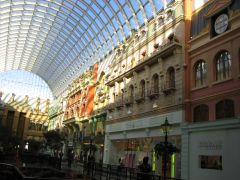
\includegraphics[width=.45\linewidth]{img/example_1}} \quad
\subfloat[Pan ma signo.]
{\label{fig:example-b}

\includegraphics[width=.45\linewidth]{img/example_2}} \\
\subfloat[Methodicamente o uno.]
{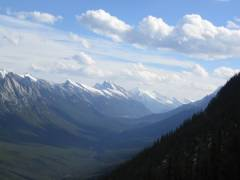
\includegraphics[width=.45\linewidth]{img/example_3}} \quad
\subfloat[Titulo debitas.]
{
\includegraphics[width=.45\linewidth]{img/example_4}}
\caption[Tu duo titulo debitas latente]{Tu duo titulo debitas latente.}\label{fig:example}
\end{figure}

